\begin{tabularx}{\textwidth}{| l | X |}
  \hline
  Datum: & 18/05/2020\\
  \hline
  Omschrijving: & \hl{Het tonen van een werkend A* zoekalgoritme in een 3D Octree. Met een uitvoerbaar pad als output, dit wilt zeggen enkel de punten die waardevolle informatie bieden.}\\
  \hline
  Resultaat: &
  \raisebox{-0.9\totalheight}{\centerline{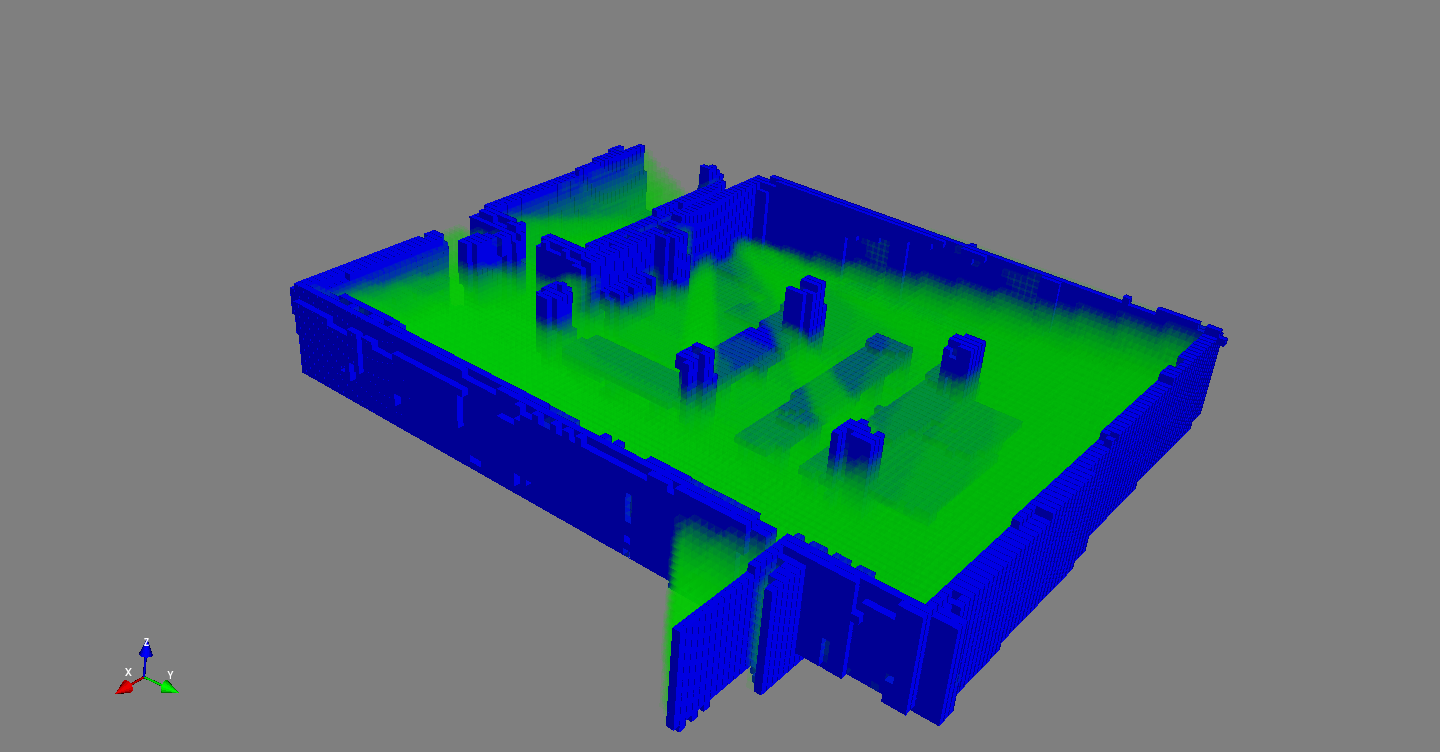
\includegraphics[width=0.65\linewidth]{demo_4/octree_visualisation.png}}}
  \raisebox{-0.9\totalheight}{\centerline{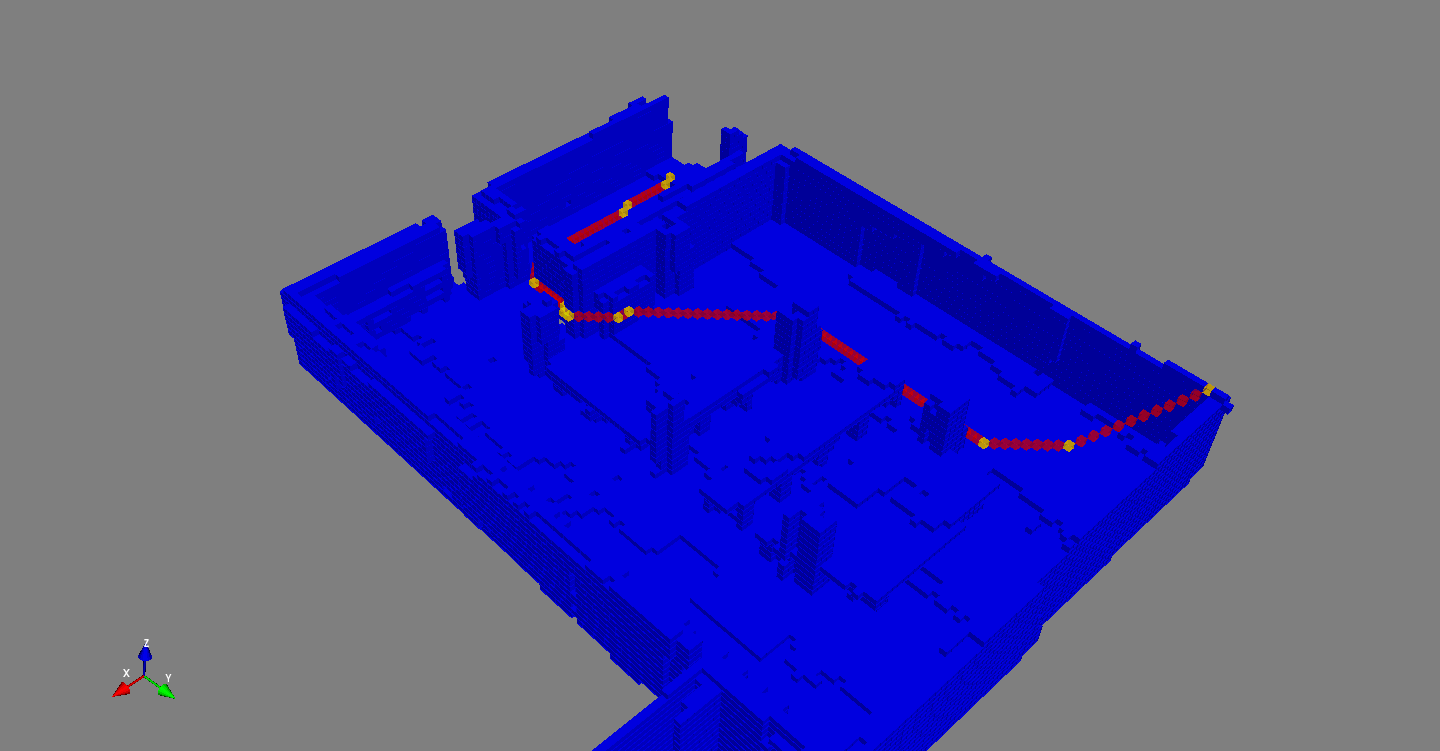
\includegraphics[width=0.65\linewidth]{demo_4/executable_path.png}}}\\
  \hline
\end{tabularx}